\documentclass{article}
\usepackage[margin=2cm]{geometry}
\usepackage{tabu}
\usepackage{mathtools}
\usepackage{enumitem}
\usepackage{amssymb}
\usepackage{newcent}
\usepackage{amsmath}
\usepackage{hyperref}


\title{COL726 Homework 3}
\author{Lovish Madaan \\ \texttt{2015CS50286}}
\date{}
\begin{document}
\maketitle

\begin{enumerate}
    \item
    \begin{enumerate}[label=(\alph*)]
        \item The LU decomposition of a banded matrix without pivoting will give L and U that are lower banded and upper banded respectively. For e.g., for $l = 2$ and $u = 1$, we have
        $$L = \begin{bmatrix}
            \times & & & & \\
            \times & \times & & & \\
            \times & \times & \times &  & \\
             & \ddots & \ddots & \ddots & \\
             & & \times & \times & \times \\
        \end{bmatrix}$$
        $$U = \begin{bmatrix}
            \times & \times &  &  & \\
             & \times & \times &  & \\
             &  & \times & \ddots & \\
             &  &  & \ddots & \times \\
             &  &  &  & \times \\
        \end{bmatrix}$$
        So, modifying the Gaussian Elimination Algorithm without pivoting using the above fact will result in the following algorithm:
        \begin{enumerate}
            \item $U = A$, $L = I$
            \item for $k = 1$ to $m - 1$
            \item $\quad\quad$for $j = k + 1$ to $min(k + l, m)$
            \item $\quad\quad\quad\quad l_{jk} = u_{jk} / u_{kk}$
            \item $\quad\quad\quad\quad u_{j, k : min(k + u, m)} = u_{j, k : min(k + u, m)} - l_{jk}u_{j, k : min(k + u, m)}$
        \end{enumerate}
        Now to count the number of flops, step \romannumeral 5 $\;$ takes at max $2u$ flops per one iteration of the inner for loop. The inner loop is computed at max $l$ times. So, the total cost of inner for loop is $2lu$ per one iteration of outer for loop. Since, the outer for loop is computed $m$ times, the total cost is $2lum$ flops.
        \item For $l = 1$ and $u = 1$, consider matrix $A$ as:
        $$A = \begin{bmatrix}
            1 & 5 & 0 & 0 & 0 \\
            6 & 1 & 4 & 0 & 0 \\
            0 & 7 & 1 & 3 & 0 \\
            0 & 0 & 8 & 1 & 2 \\
            0 & 0 & 0 & 9 & 1 \\
        \end{bmatrix}$$
        The LU decomposition with partial pivoting results in the following decomposition:
        $$P = \begin{bmatrix}
            0 & 1 & 0 & 0 & 0 \\
            0 & 0 & 1 & 0 & 0 \\
            0 & 0 & 0 & 1 & 0 \\
            0 & 0 & 0 & 0 & 1 \\
            1 & 0 & 0 & 0 & 0 \\
        \end{bmatrix}, 
        L = \begin{bmatrix}
            1 & 0 & 0 & 0 & 0 \\
            0 & 1 & 0 & 0 & 0 \\
            0 & 0 & 1 & 0 & 0 \\
            0 & 0 & 0 & 1 & 0 \\
            0.167 & 0.691 & -0.170 & -0.211 & 1 \\
        \end{bmatrix}, 
        U = \begin{bmatrix}
            6 & 1 & 4 & 0 & 0 \\
            0 & 7 & 1 & 3 & 0 \\
            0 & 0 & 8 & 1 & 2 \\
            0 & 0 & 0 & 9 & 1 \\
            0 & 0 & 0 & 0 & 0.551 \\
        \end{bmatrix}$$
    Here, $L$ has non zero value in its bottom left entry.
    \end{enumerate}
    \clearpage
    \item We have $M = \begin{bmatrix}
        A & b\\
        b^T & c
    \end{bmatrix}$ and $A = LL^T$. Let the Cholesky decomposition of $M$ be $M = \tilde{L}\tilde{L}^T$ and let $\tilde{L} = \begin{bmatrix}
        L_1 & 0\\
        d^T & e\\
    \end{bmatrix}$ where $L_1$ is some lower triangular matrix, $d$ is a vector and $e$ is a scalar.\\
    Now,
    \begin{equation}
    \tilde{L}\tilde{L}^T = \begin{bmatrix}
        L_1 & 0\\
        d^T & e\\
    \end{bmatrix}\begin{bmatrix}
        L_1^T & d\\
        0 & e\\
    \end{bmatrix} = \begin{bmatrix}
        L_1L_1^T & L_1d\\
        d^TL_1^T & d^Td + e^2
    \end{bmatrix} = \begin{bmatrix}
        L_1L_1^T & L_1d\\
        d^TL_1^T & ||d||^2 + e^2
    \end{bmatrix}
    \end{equation}
    Also, we have
    \begin{equation}
    \tilde{L}\tilde{L}^T = M = \begin{bmatrix}
        A & b\\
        b^T & c
    \end{bmatrix}
    \end{equation}
    Using (1) and (2),
    $$\begin{bmatrix}
        L_1L_1^T & L_1d\\
        d^TL_1^T & ||d||^2 + e^2
    \end{bmatrix} = \begin{bmatrix}
        A & b\\
        b^T & c
    \end{bmatrix}$$
    Since, $A$ is SPD, the Cholesky decomposition of $A$ is unique.
    So, we get
    \begin{equation}
    L = L_1
    \end{equation}
    \begin{equation}
    L_1d = b \Rightarrow Ld = b
    \end{equation}
    \begin{equation}
    ||d||^2 + e^2 = c \Rightarrow e = \sqrt{c - ||d||^2}
    \end{equation}
    Equation (4) can be solved for d in $O(m^2)$ time using forward substitution since $L$ is lower triangular.
    $$\begin{bmatrix}
        l_{11} & & & \\
        l_{21} & l_{22} & & \\
        \vdots & & \ddots & \\
        l_{m1} & \cdots & & l_{mm}
    \end{bmatrix}\begin{bmatrix}
        d_1\\
        d_2\\
        \vdots \\
        d_m
    \end{bmatrix} = \begin{bmatrix}
        b_1\\
        b_2\\
        \vdots \\
        b_m\\
    \end{bmatrix}$$
    So, we get the values of $d_i$ iteratively by:
    $$l_{11}d_1 = b_1 \Rightarrow d_1 = \frac{b_1}{l_{11}}$$
    $$l_{21}d_1 + l_{22}d_2 = b_2 \Rightarrow d_2 = \frac{b_2 - l_{21}d_1}{l_{22}}$$
    $$\vdots$$
    $$l_{m1}d_1 + \cdots + l_{mm}d_m = b_m \Rightarrow d_m = \frac{b_m - l_{m1}d_1 - \cdots - l_{m(m - 1)}d_{m - 1}}{l_{mm}}$$
    Once we have $d$, we can get the value of $e$ using equation (5). Using the values of $L$, $d$ and $e$, we can get $\tilde{L} = \begin{bmatrix}
        L & 0\\
        d^T & e
    \end{bmatrix}$.
    \clearpage
    \item 
    \begin{enumerate}[label=(\alph*)]
    \item First decompose $A$ into $A = D + L + U$, where $D$ is formed from the diagonal entries of $A$, $L$ is formed using the matrix entries of $A$ below the diagonal and $U$ is formed using the matrix entries of $A$ above the diagonal.
    Now, $Ax = b$ can be written as $(D + L + U)x = b$, or simply:
    $$Dx = b - (L + U)x$$
    $$x = D^{-1}b - D^{-1}(L + U)x$$
    Here $x$ is a fixed point that satisfies the above equation. So, we can write the update rule as:
    $$x^{(n + 1)} = D^{-1}(b - (L + U)x^n)$$
    This iterative method is the Jacobian stationary iterative method.
    \item The update rule using for loop in this case can be written as:
    $$x_{q_k} \leftarrow \frac{1}{a_{p_kq_k}}(b_{p_k} - \sum\limits_{j \neq q_k}a_{p_kj}x_j)$$
    First form permutation matrices $P$ and $Q$ from $(p_1, \cdots, p_m)$ and $(q_1, \cdots, q_m)$ respectively. For e.g. for $m = 4$ and $(p_1, p_2, p_3, p_4) = (3, 1, 4, 2)$, we have:
    $$P = \begin{bmatrix}
        0 & 0 & 1 & 0 \\
        1 & 0 & 0 & 0 \\
        0 & 0 & 0 & 1 \\
        0 & 1 & 0 & 0 \\
    \end{bmatrix}$$
    Now, we will do the decomposition of matrix $PAQ^T$, i.e. $PAQ^T = D' + L' + U'$. This is because we want $a_{p_kq_k}$ as the diagonal element instead of $a_{kk}$. $P$ will exchange the rows and $Q^T$ will exchange the columns. To get $b_{p_k}$ from $b_k$, we multiply by $P$. So, the update rule becomes
    $$Qx^{(n + 1)} = D'^{-1}(Pb - (L' + U')Qx^n)$$
    \end{enumerate}
    \item The Krylov subspace is written as $K_k = <q_1, q_2, \cdots, q_k> = <b, Ab, A^2b, \cdots, A^{k - 1}b>$. Since $b$ lies in the span of $n$ eigenvectors of $A$ say $v_1, v_2, \cdots, v_n$, we can write $b$ as the linear combination of these $n$ eigenvectors. i.e. $b = \sum\limits_{i = 1}^{n}\alpha_iv_i$.\\
    Now,
    $$A^jb = A^j(\sum\limits_{i = 1}^{n}\alpha_iv_i) = \sum\limits_{i = 1}^n \alpha_i(A^jv_i) = \sum\limits_{i = 1}^{n}\alpha_i\lambda_i^jv_i$$
    i.e. we can write $A^jb$ as the linear combination of $v_i$'s.\\
    Suppose Arnoldi iteration does not break for any number of iterations less than equal to $n$. This means that $A^{n}b$(formed after $n^{th}$ step) is linearly independent of the vectors forming the basis of the Krylov subspace $K_n$. Therefore, we get $n + 1$ dimensional basis for $K_{n + 1}$. But we showed that each of $A^jb$'s are linear combination of $v_1, v_2, \cdots, v_n$ thus $K_{n + 1}$ can be atmost $n$ dimensional which is a contradiction. Hence, Arnoldi iteration breaks down in at most $n$ iterations.\\

    Assume that the Arnoldi iteration breaks down after $k$ steps. Therefore $Aq_k$ lies in $K_k$. Also, $Aq_j \; \forall j < k$ lies in $K_k$(Construction of Arnoldi iteration). Now, any vector $x$ lying in $K_k$ will have $Ax$ lying in $K_k$(because $x$ can be written as a linear combination of $q_1, \cdots, q_k$).\\
    Since $A$ is full rank, it will map 2 distinct $x_i$'s in $K_k$ to distinct vectors. Therefore, there will exist a unique $x_*$ such that $Ax_* = b$. Hence, GMRES solves $\min\limits_{x \subset K_k}||Ax - b||_2$ exactly.
    \clearpage
    \item We have $||A - I||_2 = 0.6$
    \begin{enumerate}[label=(\alph*)]
        \item Using the definition of induced norm, we have
        $$||A - I||_2 = \max_x \frac{||(A - I)x||_2}{||x||_2} = \max_x\frac{||Ax - x||_2}{||x||_2}$$
        Now, suppose $v$ is an eigenvector of $A$ with eigenvalue $\lambda$. We have
        \begin{equation}
        Av = \lambda v
        \end{equation}
        \begin{equation}
        \frac{||Av - v||_2}{||v||_2} \leq \max_x\frac{||Ax - x||_2}{||x||_2}
        \end{equation}
        Put (6) in (7) to get
        $$\frac{||\lambda v - v||_2}{||v||_2} \leq \max_x\frac{||Ax - x||_2}{||x||_2}$$
        Therefore,
        $$\frac{||\lambda v - v||_2}{||v||_2} = \frac{|\lambda - 1|\;||v||_2}{||v||_2} = |\lambda - 1| \leq \max_x\frac{||Ax - x||_2}{||x||_2} = ||A - I||_2 = 0.6$$
        So, $|\lambda - 1| \leq 0.6 \Rightarrow 0.4 \leq \lambda \leq 1.6$\\
        Since $A$ is SPD, we have
        $$\frac{||e_n||_A}{||e_0||_A} \leq 2 (\frac{\sqrt{\kappa} - 1}{\sqrt{\kappa} + 1})^n$$
        where $\kappa = ||A||_2 = \frac{|\lambda_{max}|}{|\lambda_{min}|} \leq \frac{1.6}{0.4} = 4$\\
        Therefore using the fact that $\frac{\sqrt{\kappa} - 1}{\sqrt{\kappa} + 1}$ is an increasing function,
        $$\frac{||e_n||_2}{||e_0||_2} \leq 2 (\frac{\sqrt{\kappa} - 1}{\sqrt{\kappa} + 1})^n \leq 2 (\frac{\sqrt{4} - 1}{\sqrt{4} + 1})^n = \frac{2}{3^n}$$
        \item We have $B = A + ww^T = A + 49v_1v_1^T$. Now, suppose $v$ is any eigenvector of $A$ with eigenvalue $\lambda$. So,
        $$Bv = (A + 49v_1v_1^T)v = Av + 49(v_1v_1^T)v = \lambda v + 49v_1(v_1^Tv) = \lambda v + 49(v_1^Tv)v_1$$
        Suppose $rank(A) = m$. Now since $A$ is SPD, $A$ will have $m$ linearly independent eigenvectors(Trefethen \& Bau's Theorem 24.5).\\
        Therefore, given 2 different eigenvectors $v_i$ and $v_j$ of $A$, we have $v_i^Tv_j = 0$. So,
        $$Bv = \lambda v + 49(v_1^Tv)v_1 = \begin{cases}
            \lambda v & v \neq v_1\\
            50v & v = v_1(||v_1||_2 = 1, \lambda_1 = 1)\\
        \end{cases}$$
        Since $v$ is an eigenvector of $A$, $v$ is an eigenvector of $B$. Only 1 eigenvalue is different for $B$ and $A$. $\lambda'_1 = 50$ and $\lambda'_i = \lambda_i \; \forall i = 2, 3, \cdots, m$, where $\lambda'_i$'s and $\lambda_i$'s are the eigenvalues of B and A respectively.
    \item \textbf{NOTE:} Used stack overflow as reference for the idea(\href{https://math.stackexchange.com/questions/1554314/improved-error-estimate-for-conjugate-gradient-method?rq=1}{Link})\\
    Using Trefethen \& Bau's Theorem 38.3, we have:
    $$\frac{||e_n||_B}{||e_0||_B} \leq \min_{p \subset P_n}\max_{\lambda \subset \Lambda(B)}|p(\lambda)|$$
    We will choose the polynomial space $Q_n$ instead of $P_n$($Q_n \subset P_n$) such that $q(50) = q(\lambda_1) = 0$. We can do this since there is minimum over the polynomial space. i.e.
    $$\min_{p \subset P_n}\max_{\lambda \subset \Lambda(B)}|p(\lambda)| \leq \min_{q \subset Q_n}\max_{\lambda \subset \Lambda(B)}|q(\lambda)|$$
    \clearpage
    Now,
    $$q(\lambda) = (1 - \frac{\lambda}{50})q'(\lambda)$$
    where $q'(\lambda) \subset Q_{n - 1}$\\
    Therefore,
    $$\min_{q \subset Q_n}\max_{\lambda \subset \Lambda(B)}|q(\lambda)| = \min_{q' \subset Q_{n - 1}}\max_{\lambda_i \subset \Lambda(B)}|(1 - \frac{\lambda_i}{50})q'(\lambda_i)| \leq (\min_{q' \subset Q_{n - 1}}\max_{\lambda_i \subset \Lambda(B) - \lambda_1}|1 - \frac{\lambda_i}{50}|\;|q'(\lambda_i)|) = Q$$
    Further,
    \begin{equation}
    Q < \min_{q' \subset Q_{n - 1}}\max_{\lambda_i \subset \Lambda(B) - \lambda_1}|q'(\lambda_i)|
    \end{equation}
    because $0.4 \leq \lambda_i \leq 1.6 \Rightarrow 1 - \frac{\lambda_i}{50} < 1 \quad \forall i = 2, 3, \cdots, m$
    Now, we can simply use the result of Trefethen \& Bau's Theorem 38.3 for RHS of (8). i.e.
    $$\min_{q' \subset Q_{n - 1}}\max_{\lambda_i \subset \Lambda(B) - \lambda_1}|q'(\lambda_i)| \leq 2 (\frac{\sqrt{\kappa'} - 1}{\sqrt{\kappa'} + 1})^{n - 1}$$
    where $\kappa' = \frac{|\lambda_{max}|}{|\lambda_{min}|}$ and $\lambda_{max}, \lambda_{min} \subset \{\lambda_2, \lambda_3, \cdots, \lambda_m\}$
    Now, using the result from part (a), we get:
    $$\frac{||e_n||_B}{||e_0||_B} < \frac{2}{3^{n - 1}}$$
    \end{enumerate}
    \clearpage
    \item 
    \begin{enumerate}[label=(\alph*)]
        \item  The matrix $A$ will have the entries as following:
        $$a_{ij} = \begin{cases}
            (\sum\limits_{j \textrm{ connected to } i} \frac{1}{R_{ij}}) & i = j \quad \forall i \subset \{1, 2, \cdots, m - 2\}\\
            (\sum\limits_{j \textrm{ connected to } i} \frac{1}{R_{ij}}) + 1 & i = j \quad \forall i \subset \{0, m - 1\}\\
            -\frac{1}{R_{ij}} & j \textrm{ connected to } i\\
            0 & otherwise\\
        \end{cases}$$
        Also, we can observe that $a_{ji} = -\frac{1}{R_{ji}} = -\frac{1}{R_{ij}} = a_{ij}$. Therefore, the matrix A is symmetric.
        \item \texttt{cg} function implemented using the pseudocode given in Chapter 38, Trefethen \& Bau. On running \texttt{cg} on \texttt{makeNetwork('random1', 1000)}, we get the following plot for $||r_n||_2 / ||b||_2$ on a log scale as a function of $n$.
        \begin{figure}[!ht]
            \centering
            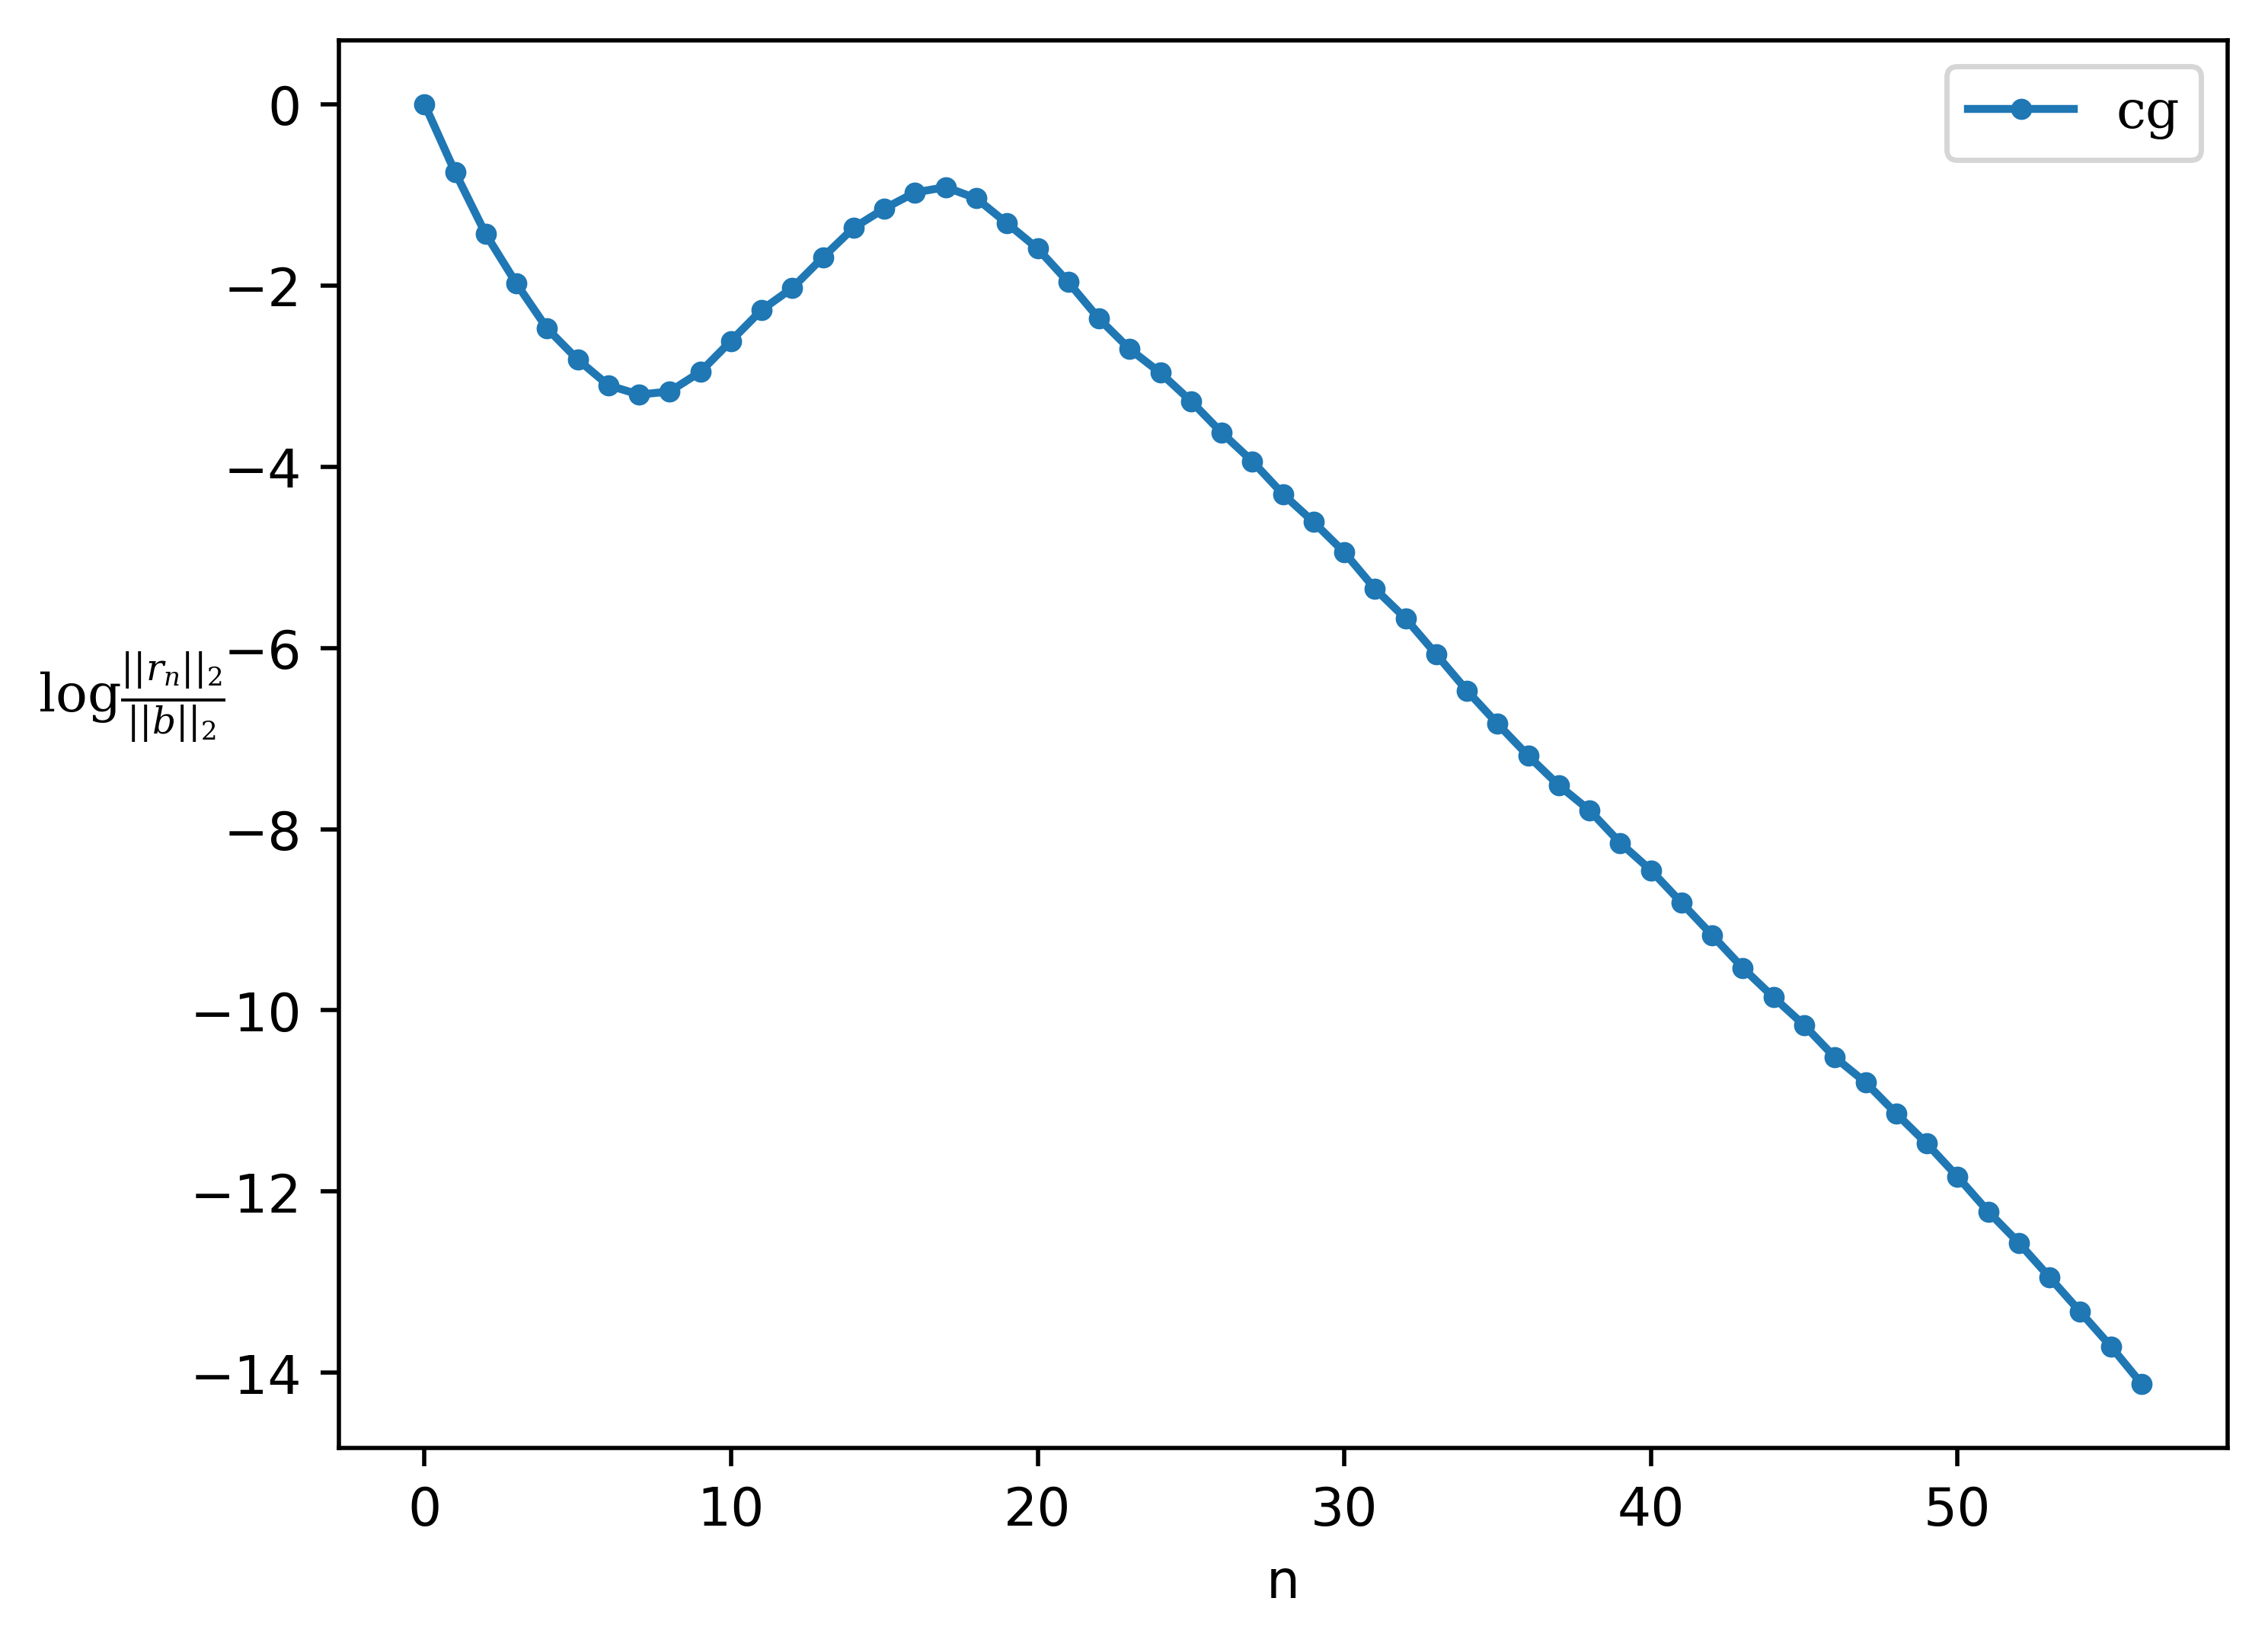
\includegraphics[scale=0.65]{fig1.png}
            \caption{$\log\frac{||r_n||_2}{||b||_2} \textrm{ vs } n$ on \texttt{makeNetwork('random1', 1000)}}
        \end{figure}
        \item Comparison of \texttt{cg} and \texttt{pcg} on \texttt{makeNetwork('random2', 1000)}.
        \begin{figure}[!ht]
            \centering
            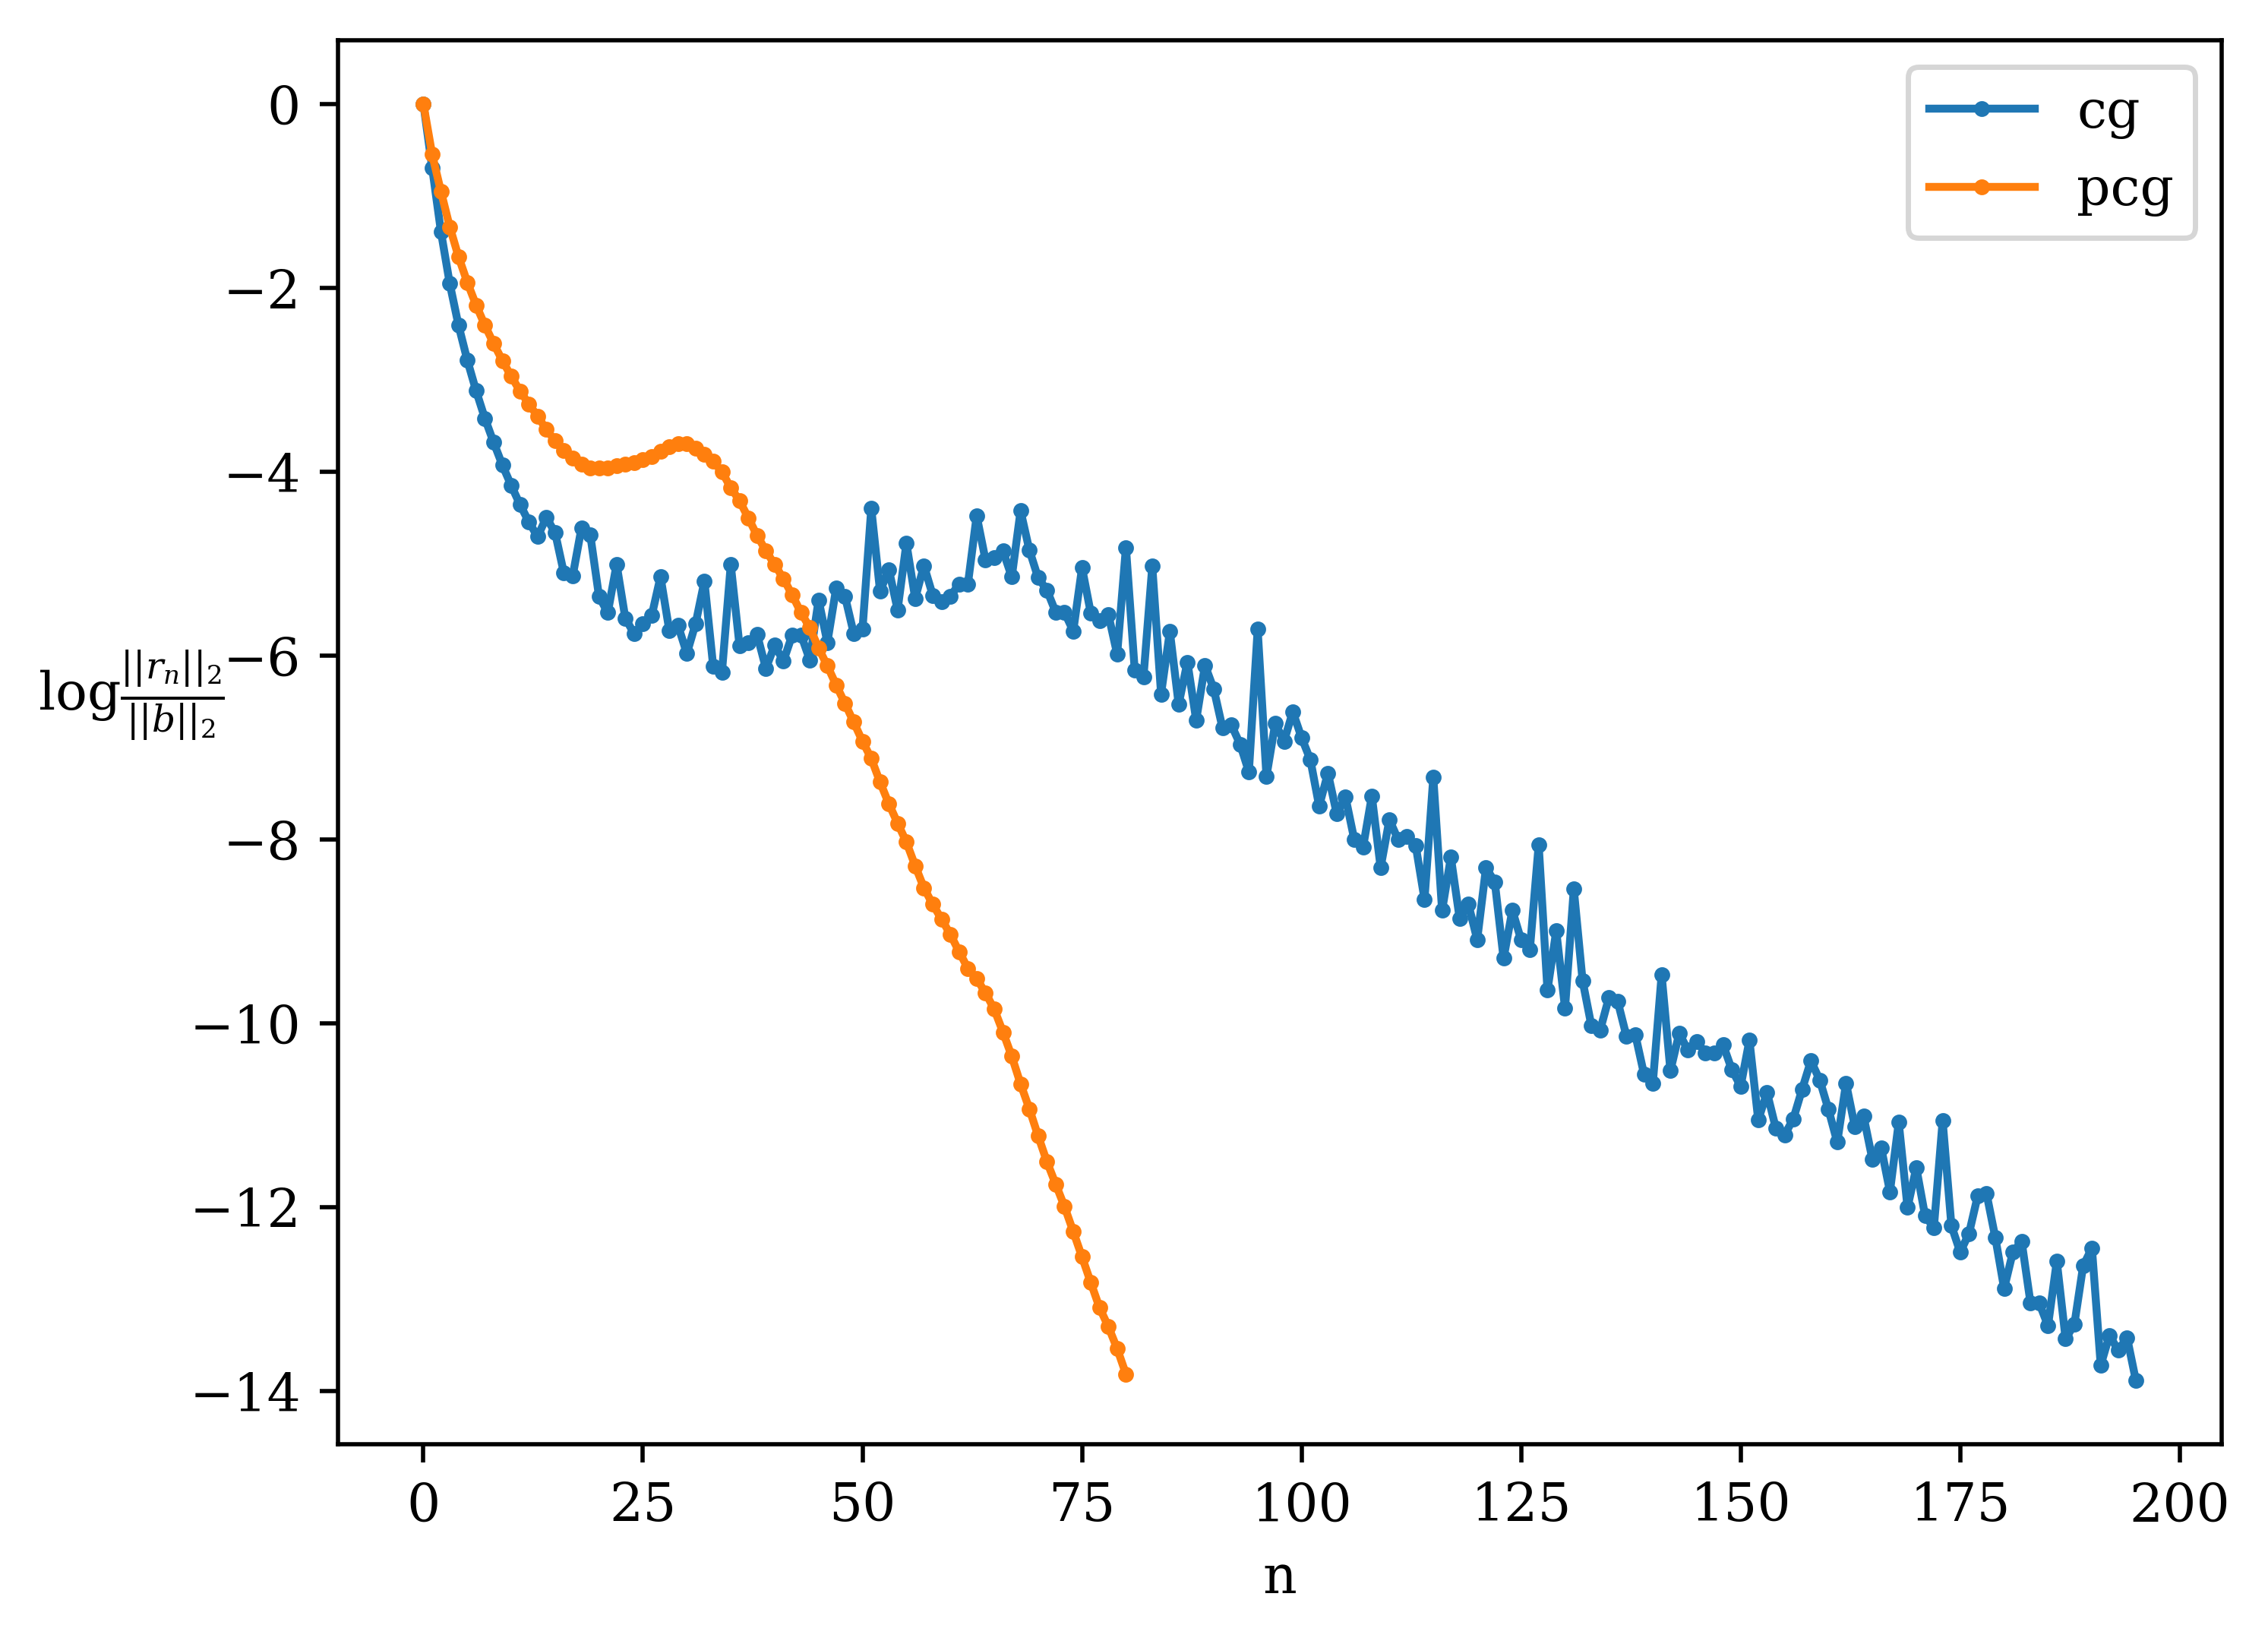
\includegraphics[scale=0.65]{fig2.png}
            \caption{$\log\frac{||r_n||_2}{||b||_2} \textrm{ vs } n$ on \texttt{makeNetwork('random2', 1000)}}
        \end{figure}
    \end{enumerate}
\end{enumerate}

\end{document}